\documentclass[]{article}

\usepackage{hyperref}
\usepackage[]{graphicx}

\hypersetup{
    colorlinks=true,
    linkcolor=blue,
    filecolor=magenta,      
    urlcolor=blue,
    pdftitle={Day 4},
    pdfpagemode=FullScreen,
    pdfauthor={Taraash},
}

\title{Week 2 Recap \\ Part 2}
\author{Taraash}
\date{}

\setcounter{secnumdepth}{0}

\begin{document}
	\maketitle
	
	\tableofcontents
	
	\newpage
	
	\section{Introduction}
	This is in continuation of \href{https://drive.google.com/file/d/1vT4dVOcDQfwohWIkxxJBOOMfCcRMoxMm/view?usp=sharing}{part 1}. Here, I will cover 
	\begin{enumerate}
		\item Event nodes
		\item Collision and overlaps
		\item Custom events
		\item Casting/interfaces
	\end{enumerate} 
	And probably some more stuff. But first, I'll list down my solution for the task I gave, if you haven't yet attempted it, I recommend skipping this part and try it out first.
	
	\section{The Task}
	Firstly, I created a blueprint (of the actor class, remember, we're just placing the door) and added my static meshes (the door and its frame).
	
	\begin{figure}[h]
		\centering
		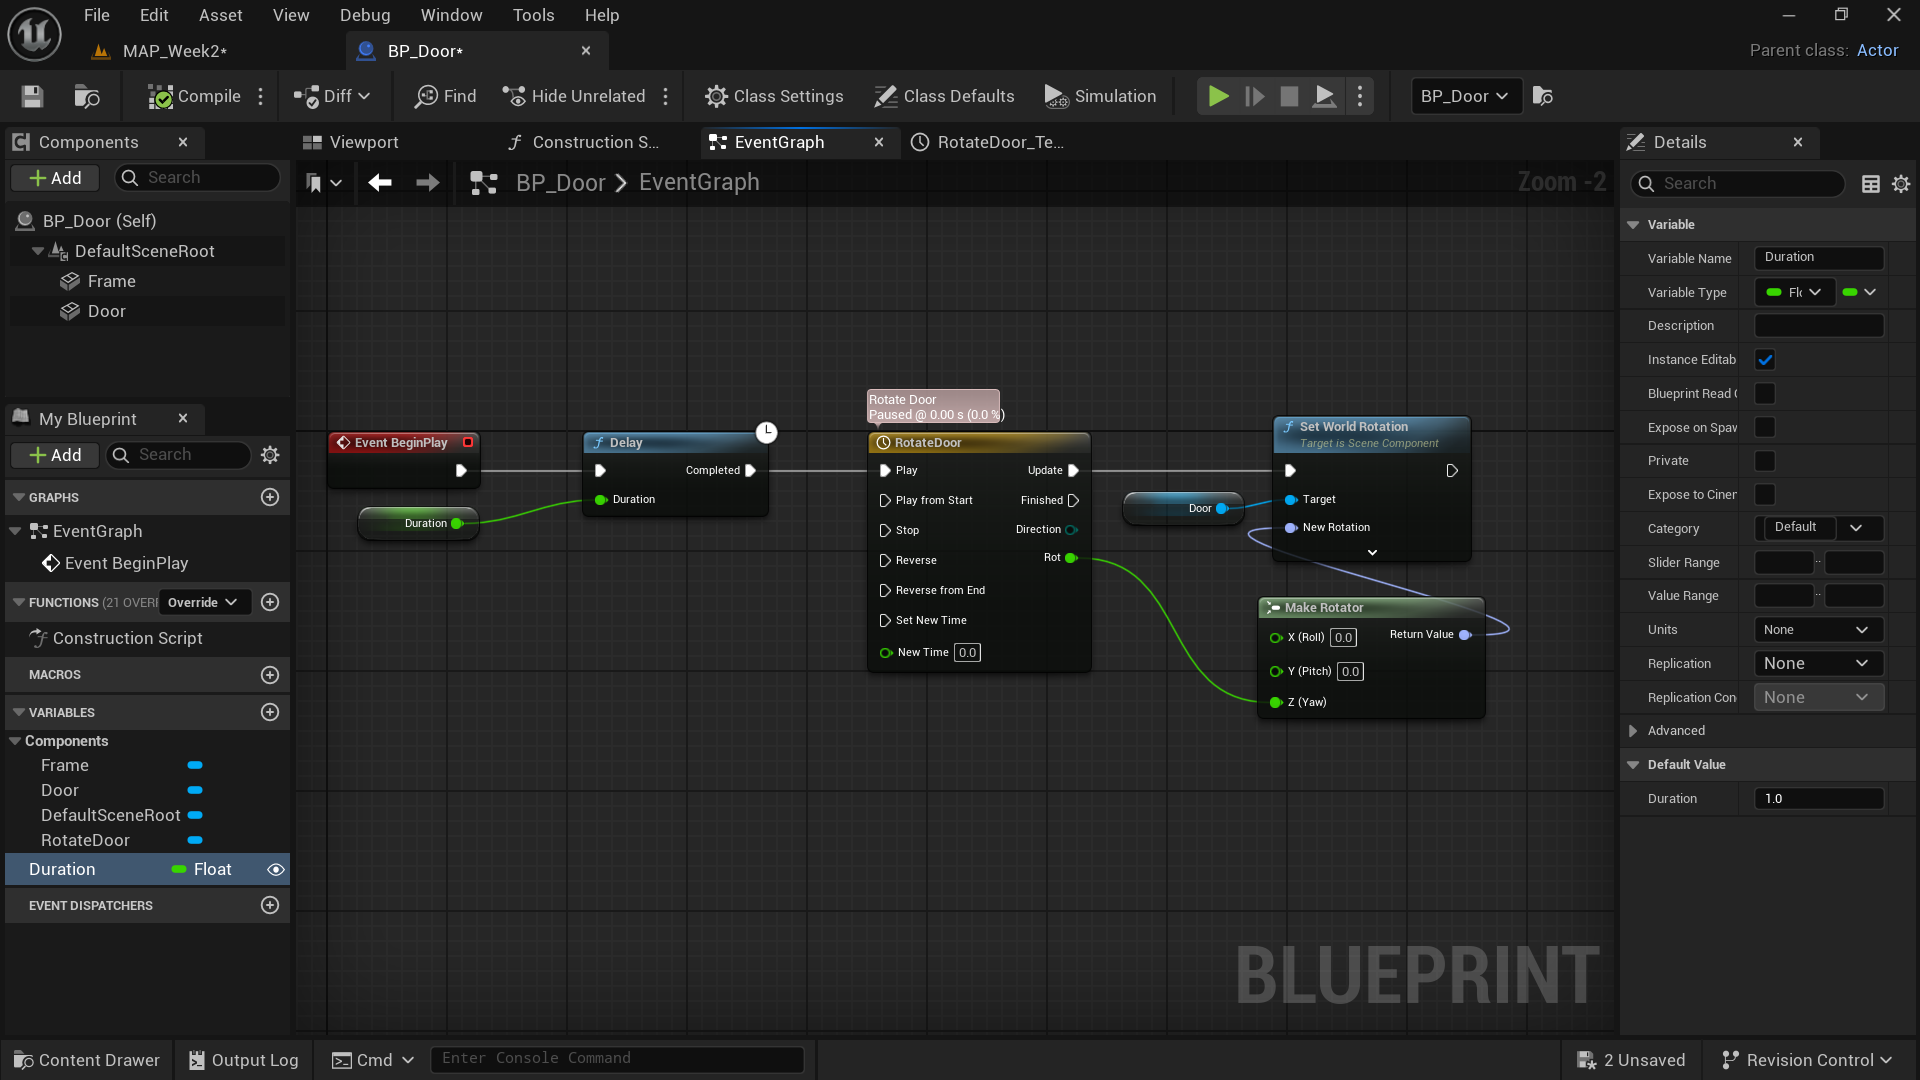
\includegraphics[width=1\linewidth]{day4images/screenshot001}
		\caption{A blueprint}
		\label{fig:screenshot001}
	\end{figure}
	
	I've added a delay node (and set the delay as a variable so we can change it), after the begin play event (I'll talk about events very soon). This ensures the door starts moving right after the number of seconds mentioned in the \verb*|Duration| parameter.
	
	\newpage
	
	\begin{figure}[h]
		\centering
		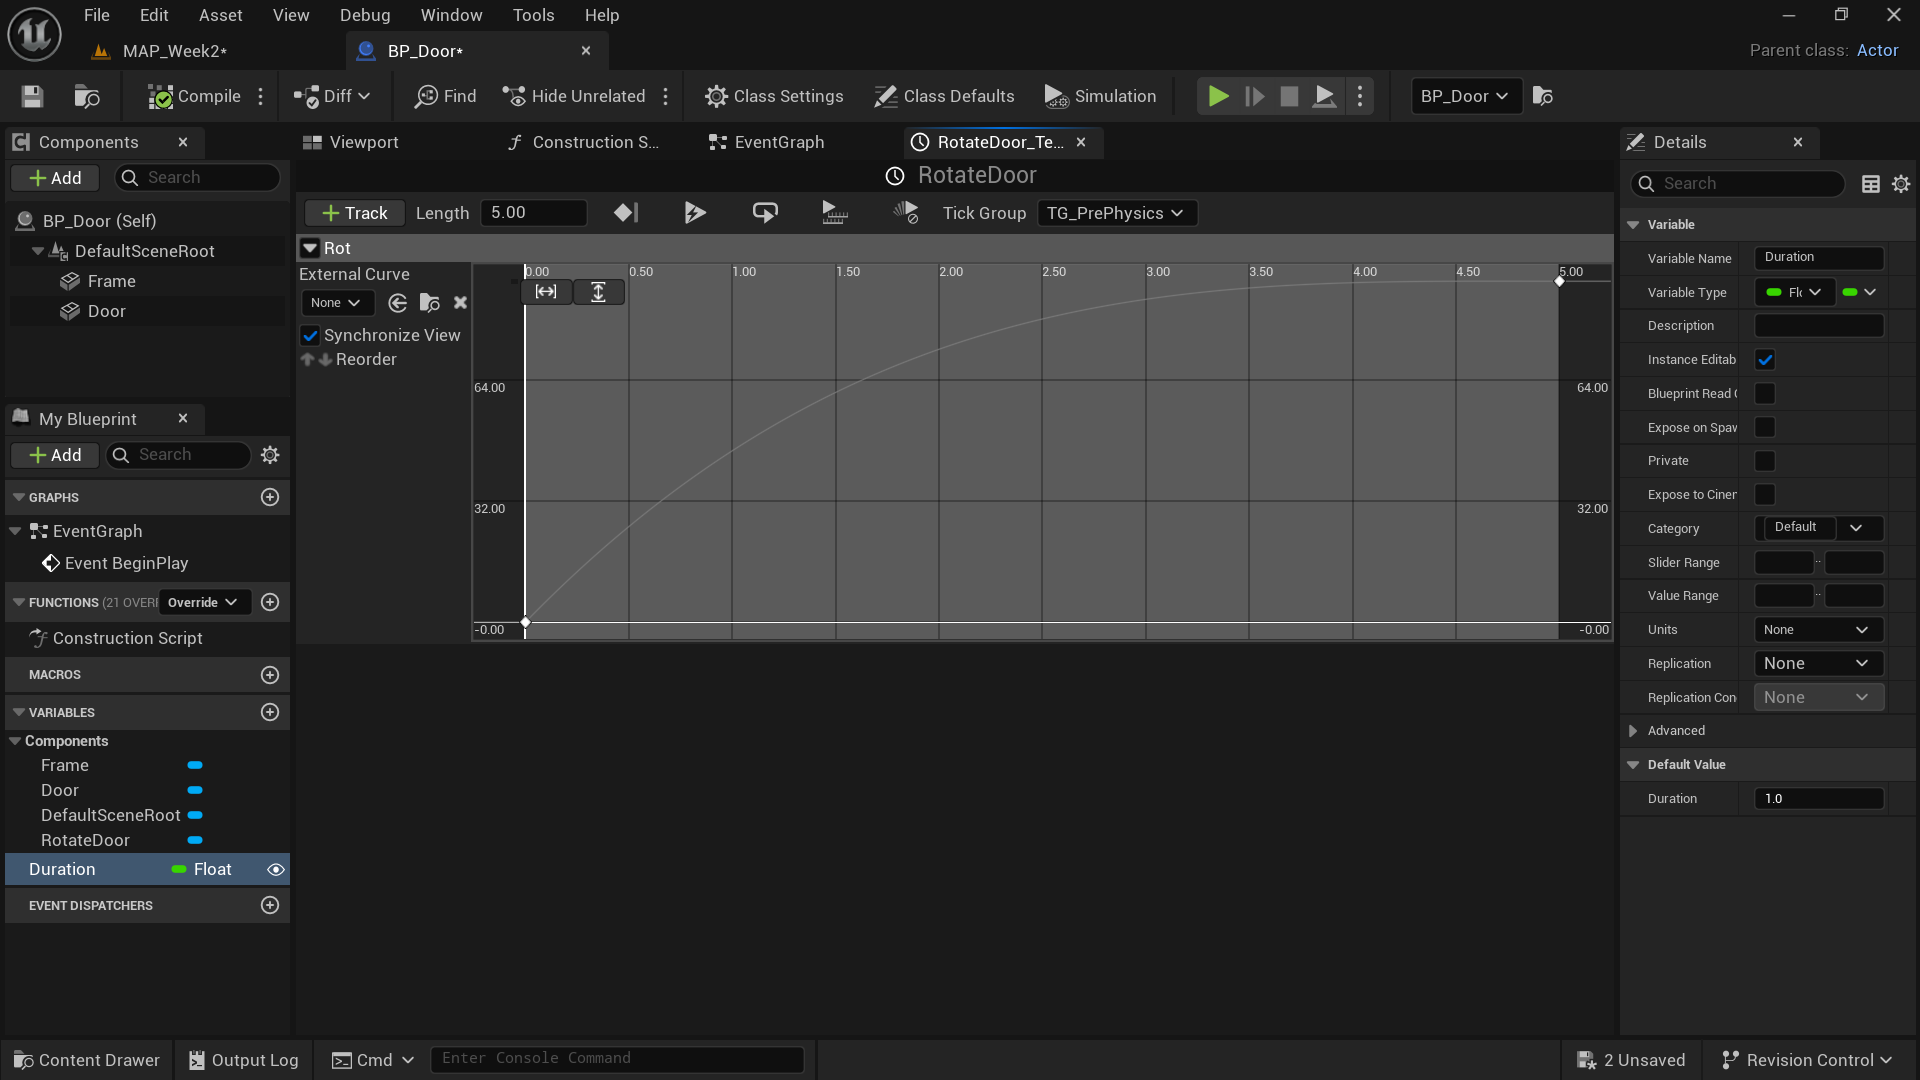
\includegraphics[width=1\linewidth]{day4images/screenshot002}
		\caption{The timeline}
		\label{fig:screenshot002}
	\end{figure}
	
	This is what the timeline node looks like, I set the easing to automatic and dragged the sliders to change the graph (it's almost never recommended to keep the default ease-in ease-out behavior, it's a little too artificially perfect). \\[10pt] I've added two key-frames, one at the start (time 0, value 0) and one at the end (as defined by the \verb*|Length| parameter on top) as (time 5, value 90). \\[10pt] We now have the ability to get from 0 to 90 in 5 seconds after the initial 1 second delay of starting the game.
	Some important notes:
	\begin{enumerate}
		\item I'm setting its absolute (world) rotation and not it's local (relative) one as at the end we want to door to be rotated by $\deg{90}$. Try using the relative node and see if you can explain why it's moving so fast.
		\item You'll also get an error the first time you run this telling you to set the door to be Movable. You do that in the Mobility section, under Transform.
		\begin{figure}[h]
			\centering
			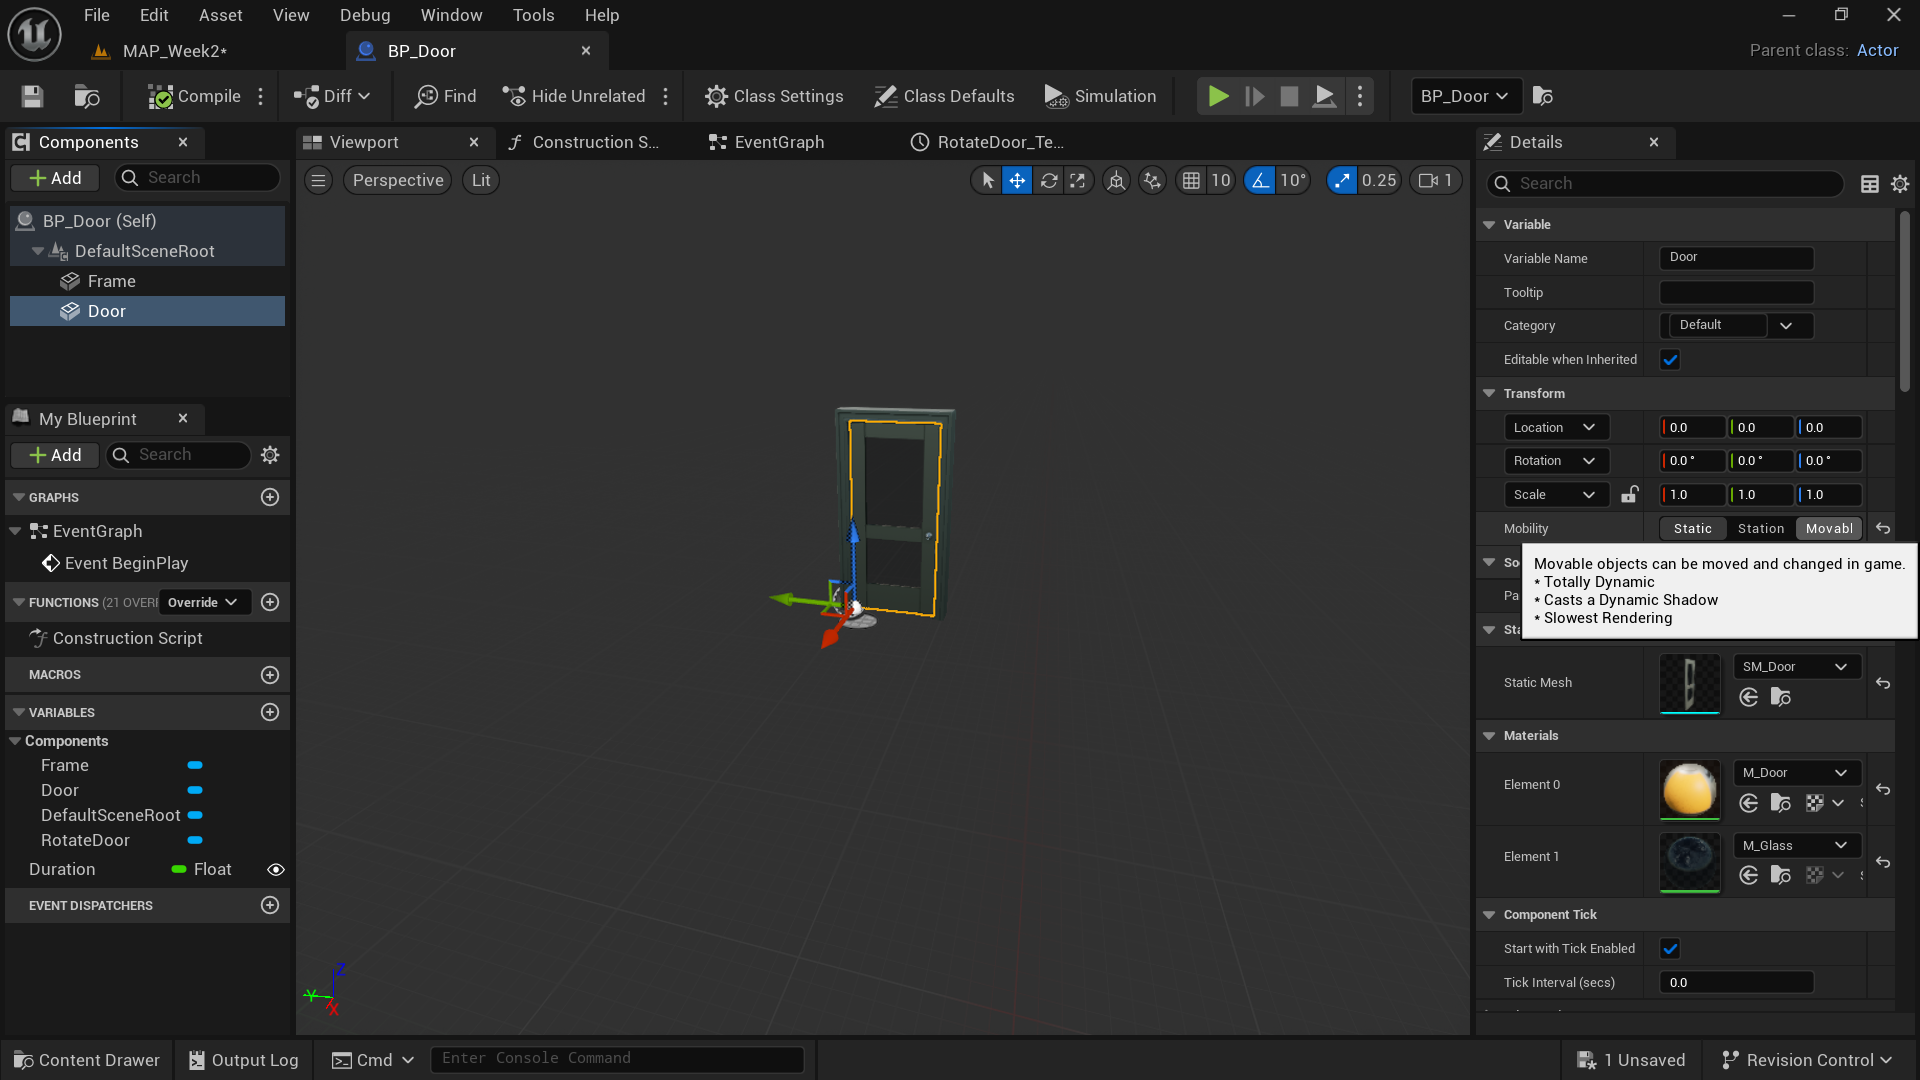
\includegraphics[width=1\linewidth]{day4images/screenshot003}
			\caption{Mobility}
			\label{fig:screenshot003}
		\end{figure}
		
	\end{enumerate}
	\newpage
	And that's pretty much it, let's now talk in detail about Events.
	

	
	\section{Events}
	Events are a set of nodes (with a red ribbon) that emit an event. Very similar to events and event listeners in JavaScript if that helps.
	\begin{figure}[h!]
		\centering
		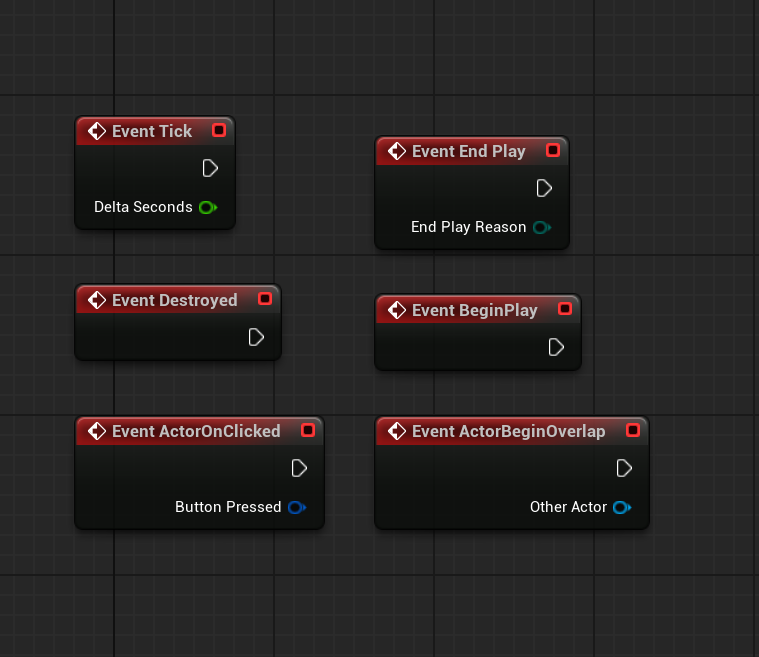
\includegraphics[width=0.6\linewidth]{day4images/screenshot005}
		\caption[]{Some event nodes}
		\label{fig:screenshot005}
	\end{figure}
	
	\newpage
	
	These send a pulse down a chain, connected via that top triangular white pin that execute the nodes in order the signal is received.
	
	That's pretty much it, there are some special event nodes that `get alive' when something particular happens, such as a collision or an overlap, and we'll talk about those now.
	
	\section{Collision and overlap events}
	 
	Remember the collider we added to our door in the static mesh editor? Doing this also enabled us to know exactly when and by who it was hit (and more information), let's take a look at it.
	
	\subsection{On Component Hit}
	I added a simple box collision to my frame and removed the code that rotated the door within. Take a look at the following screenshot:
	
	\begin{figure}[h]
		\centering
		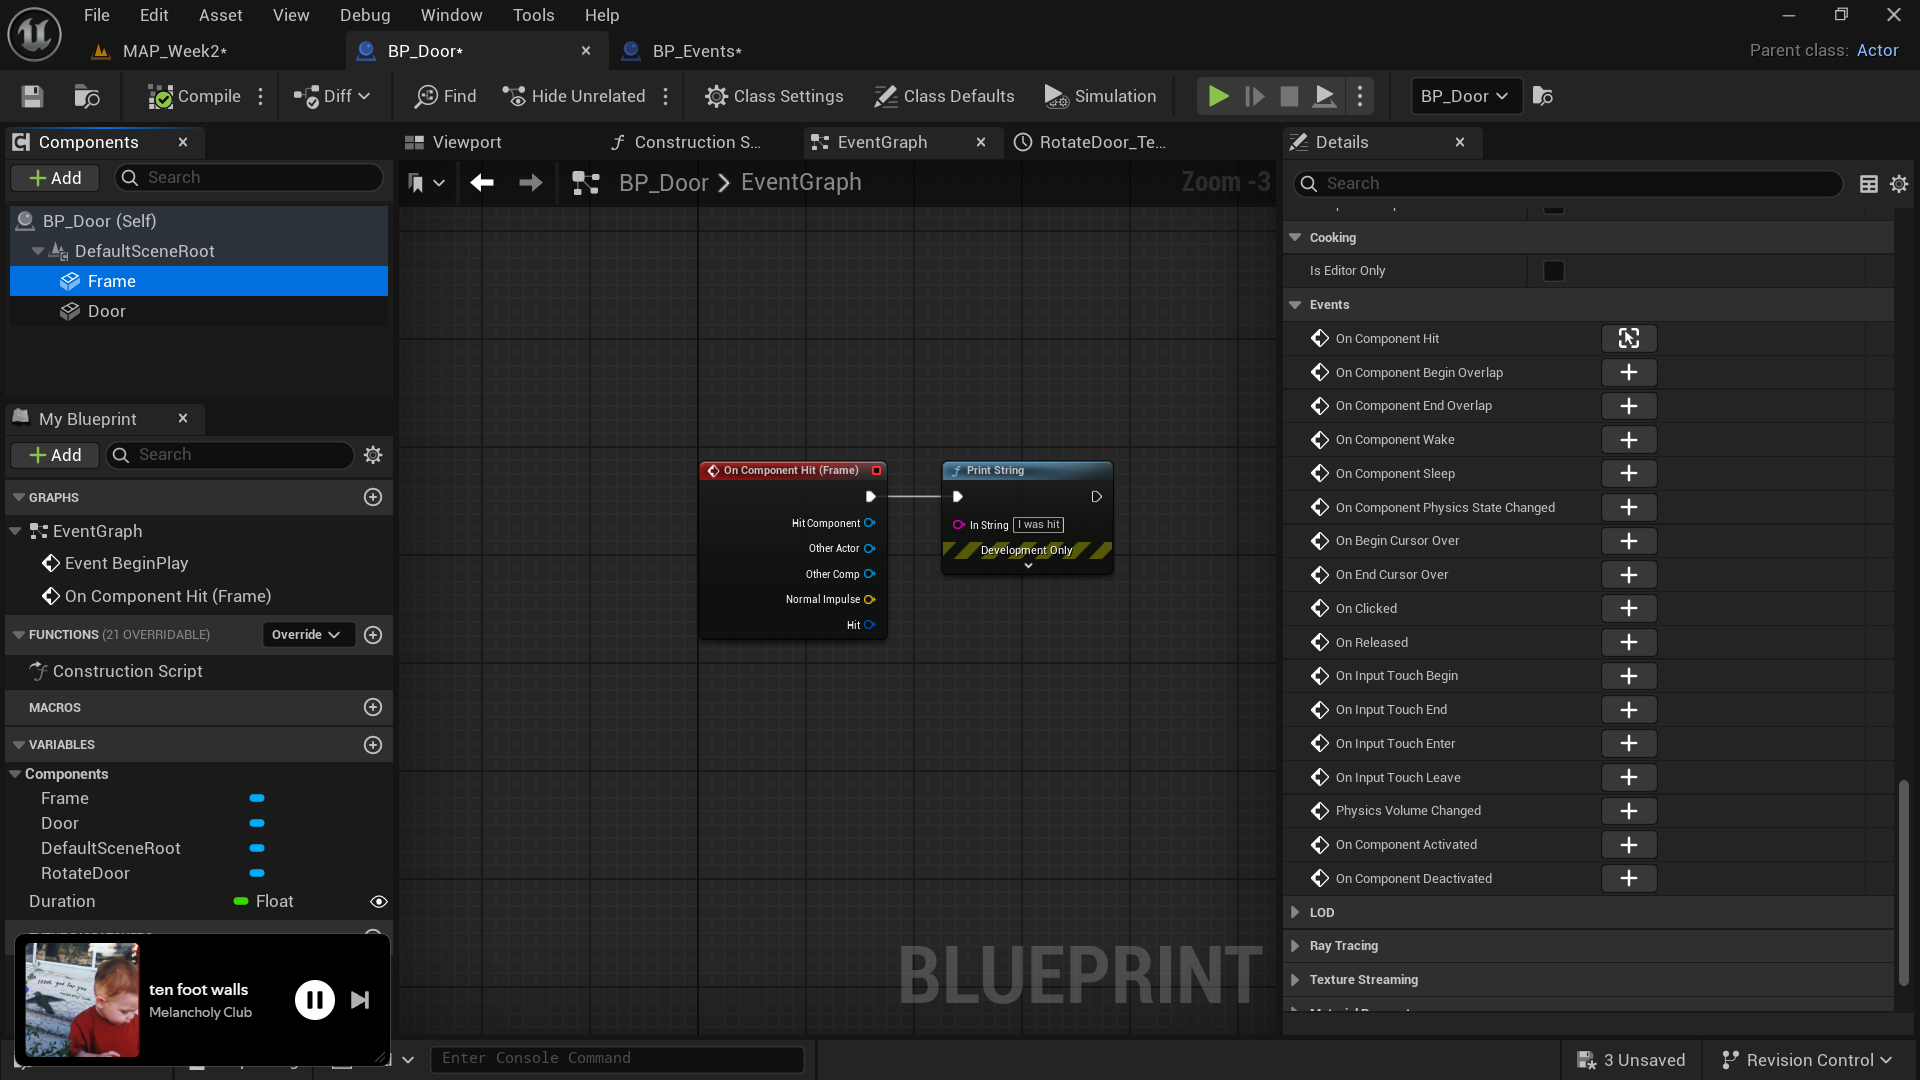
\includegraphics[width=1\linewidth]{day4images/screenshot007}
		\caption{Events per object and the component hit node}
		\label{fig:screenshot007}
	\end{figure}
	
	Let me break this down.
	\begin{enumerate}
		\item I said I added the collision box on the frame so I have that selected.
		\item With it selected, if I scroll down a little in the details panel I see a bunch of events, with the first one being the On Component Hit, press the $+$ button to add it in.
		\item The print string is just for validation, try colliding with the door now.
	\end{enumerate}
	
	Now, say we want the door to rotate whenever we hit it, if try to add a small rotation to it right now (after the print node), it won't work since we won't be able to continue moving (we're still colliding, the frame isn't moving!). We can fix this in two different ways.
	\begin{description}
		\item[In the static mesh editor] We can keep the collision mesh in the static mesh editor, there are many different ways to do so, I'll cover those later. Doing so severely limits our flexibility.
		\item[In the blueprint] We can add a simple collider mesh directly in Blueprints, this allows us to change the parameters (dimension, location etc.) dynamically.
	\end{description}
	
	\begin{figure}[h]
		\centering
		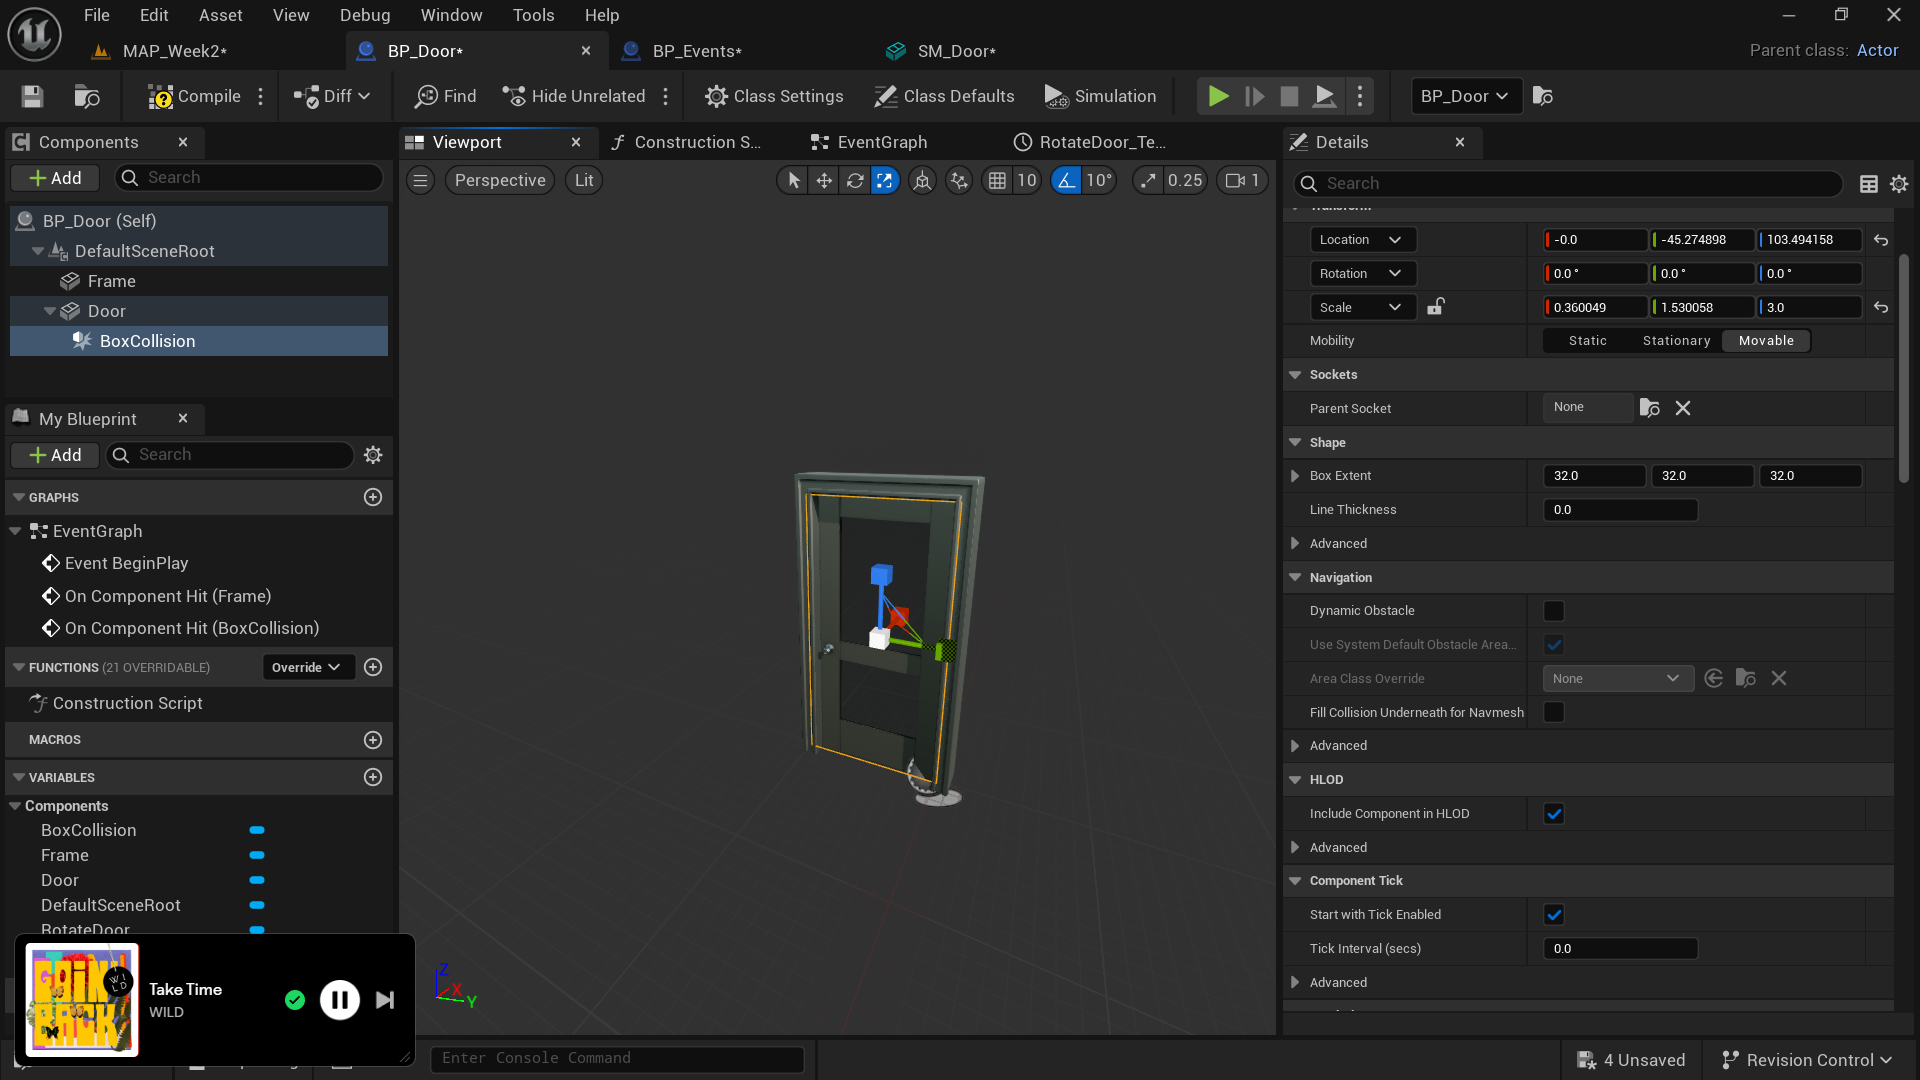
\includegraphics[width=1\linewidth]{day4images/screenshot008}
		\caption{Box collision}
		\label{fig:screenshot008}
	\end{figure}
	
	Here, I've added a box collision actor from the outliner (with our door selected, so it becomes the child, and hence, moves with the door). I then scaled and positioned it where seemed fit. Let's now add a simple rotation to this when it's hit.
	
	\newpage
	
	\begin{figure}[h]
		\centering
		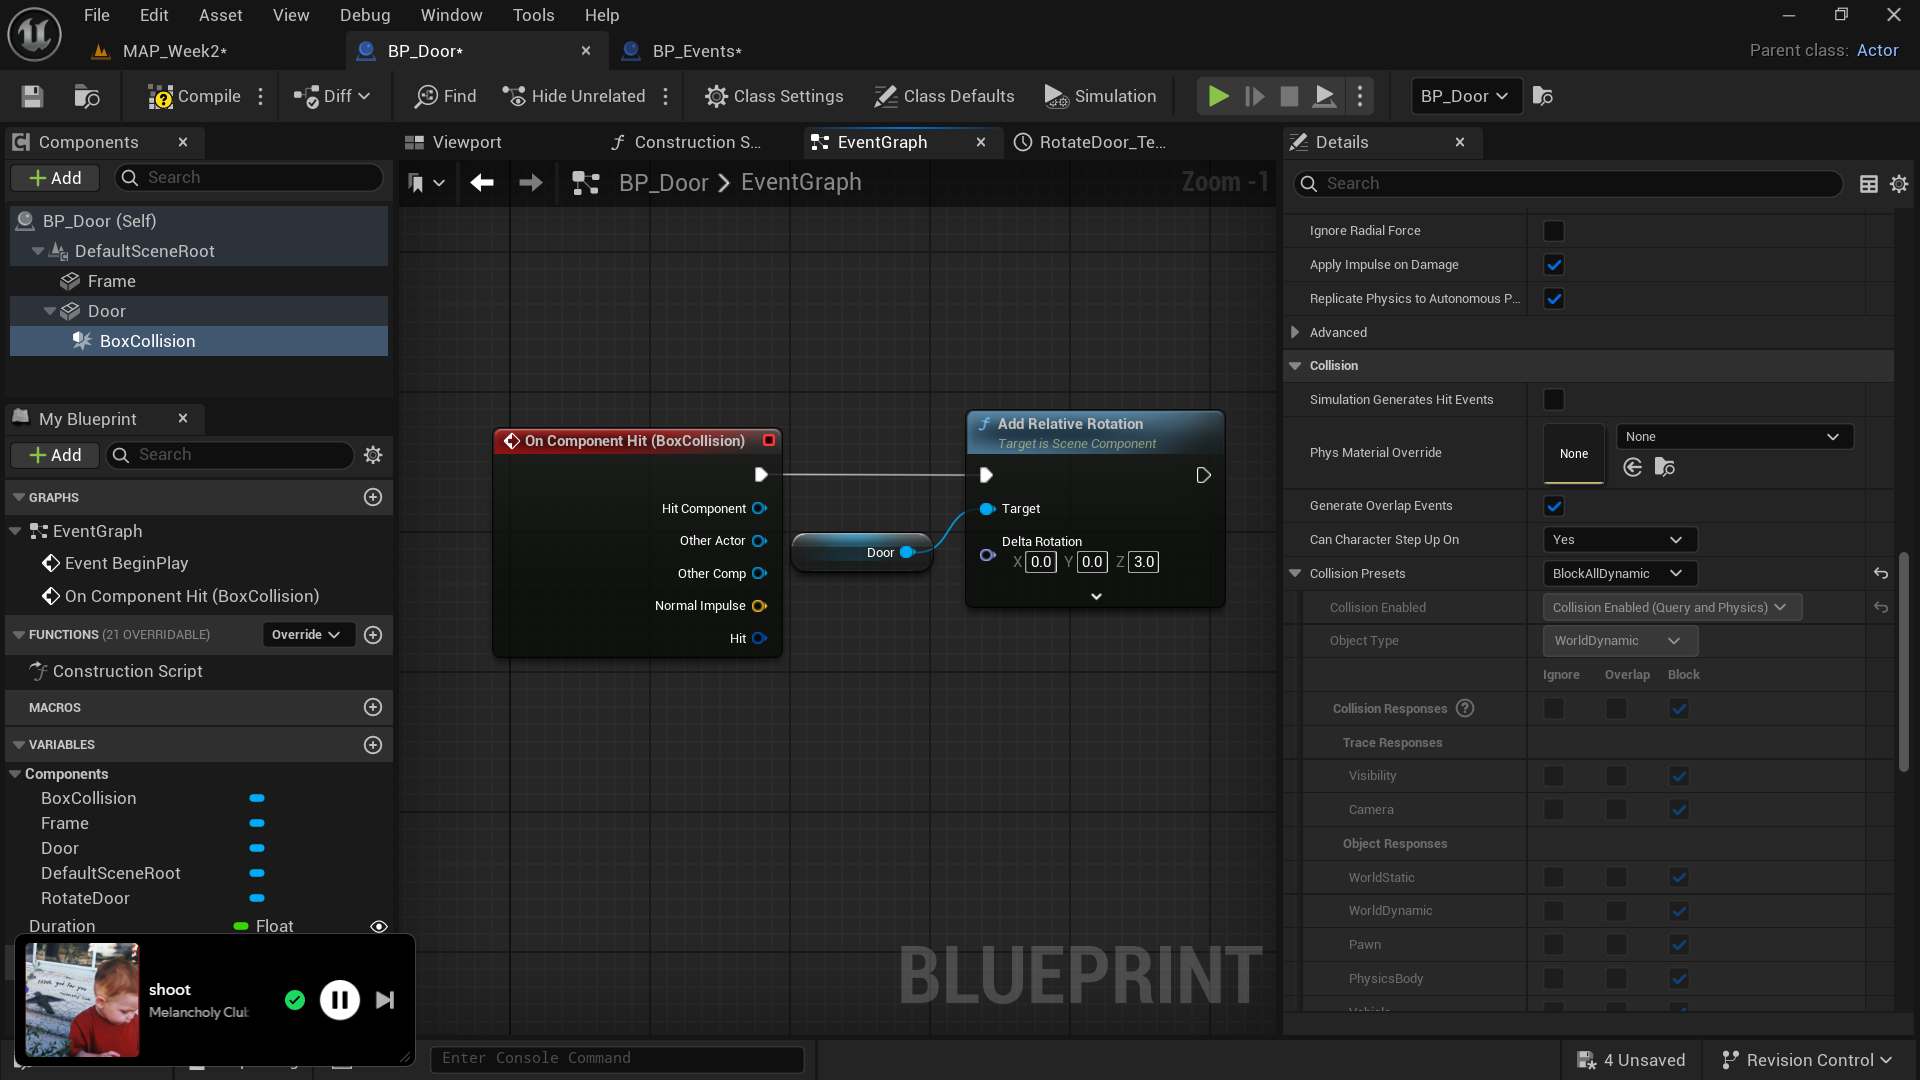
\includegraphics[width=1\linewidth]{day4images/screenshot009}
		\caption{Something simple}
		\label{fig:screenshot009}
	\end{figure}
	
	You would've immediately ran into a few problems.
	\begin{itemize}
		\item Make sure to disable the collision we added to the frame! Go to the collision tab in the static mesh editor and select \verb|No Collision|.
		\item The BoxCollision we added defaults to generating/emitting an event when someone starts or finishes overlapping it, and not when it's hit. Let's talk in more detail about this.
	\end{itemize}
	
	\subsubsection{Collision Presets}
	Take a look at the \verb|Collision Preset| setting in the details panel on the left in the above screenshot. It will be (be default) set to \verb*|OverlapAllDynamic| which means it will generate overlap events (which we will use soon!). Setting it to \verb*|BlockAllDynamic| will actually block our character and give us an event whenever we hit it. There are many more presets here, but we will mostly just use the two I've described here.
	\newpage
	Our stuff now works as expected. One quality of life we can have is the door move in the direction it is being pushed, right now we're adding a constant amount, no matter which side it is being hit from. \\[10pt] We get a very useful value, the \verb*|HitNormal| is we split the \verb*|Hit| struct (right click it and select \verb|Split Struct Pin|).
	
	\begin{figure}[h]
		\centering
		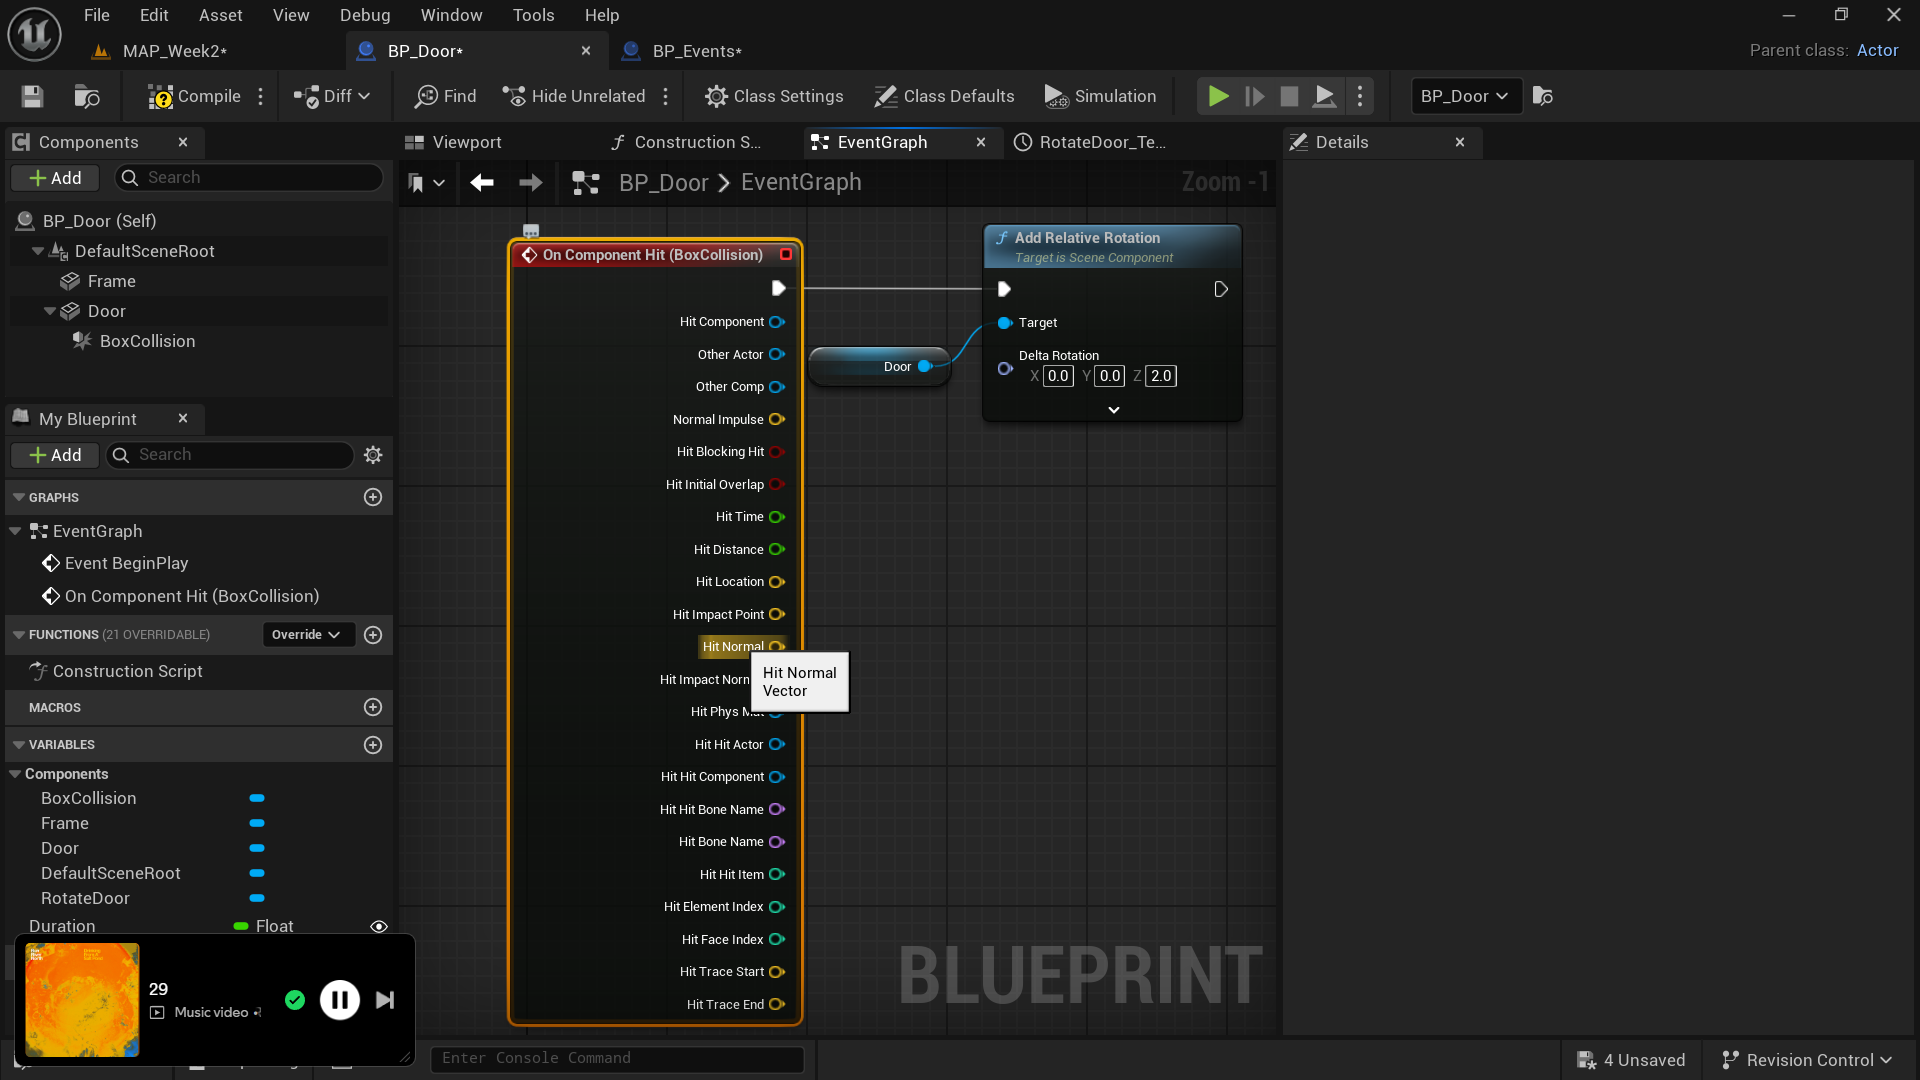
\includegraphics[width=1\linewidth]{day4images/screenshot010}
		\caption{Expanding the Hit struct to get the Hit Normal}
		\label{fig:screenshot010}
	\end{figure}
	
	(\textit{Note:} struct is exactly similar to structs in C, a collection of simpler objects/data types that are grouped in a meaningful fashion)
		\newpage
	We could print this HitNormal and see what sign corresponds to which direction and hard-code this logic, but there's a better way:

	\begin{figure}[h]
		\centering
		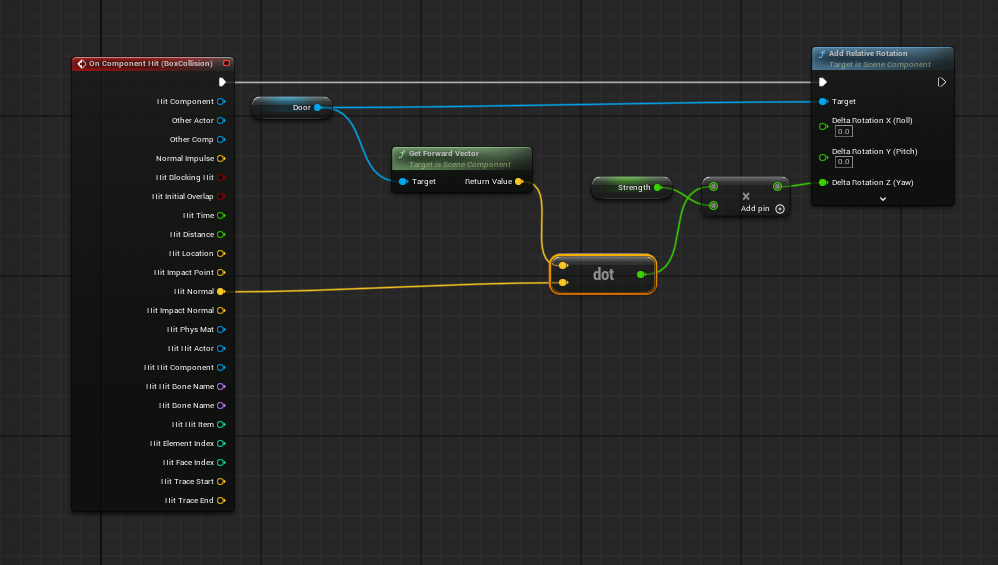
\includegraphics[width=1\linewidth]{day4images/screenshot011}
		\label{fig:screenshot011}
	\end{figure}
	
	The ForwardVector is a self-explanatory name, it's an arrow that points away from the surface of a mesh. Every static mesh in Unreal has one. The Hit Normal is a vector which is a vector pointing to the character from the point where it was hit. Now, recall the dot product. It's positive when the directions are same, and negative when the two vectors are pointing in opposite directions. This is exactly what we need! 
	\\[10pt]
	Also note
	\begin{description}
		\item[Roll] X component for rotation
		\item[Pitch] Y component
		\item[Yaw] Z component
	\end{description}
	\newpage
	Take a look at this incredibly... * coughs * suggestive drawing I made:
	
	\begin{figure}[h]
		\centering
		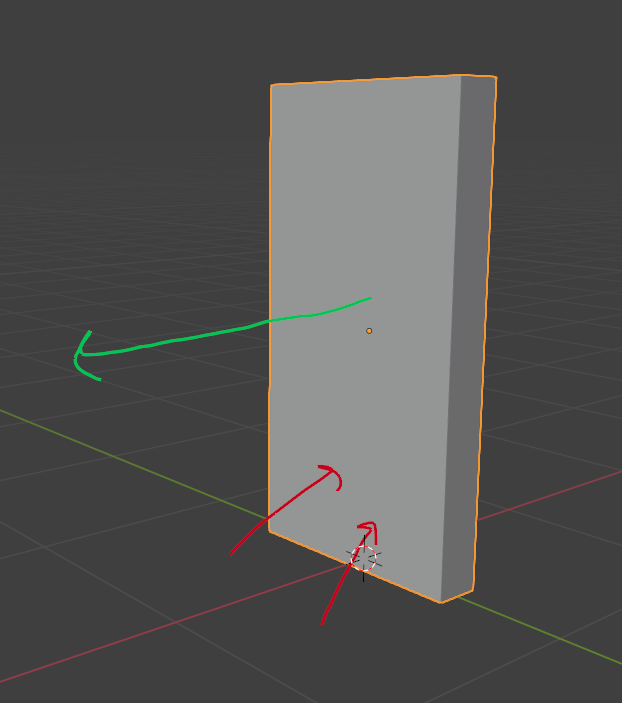
\includegraphics[width=1\linewidth]{day4images/screenshot012}
		\caption{Could NOT have done a better job}
		\label{fig:screenshot012}
	\end{figure}
	
	\begin{enumerate}
		\item The green vector is the ForwardVector
		\item The red ones are candidates for the HitNormal, can you now understand how this helps us? Dot products are very useful in the 3D world!
	\end{enumerate}
	
	We now have a functional door! Of course, depending on the style you wanna go you might want something else, perhaps pressing E to open? Let's take a look at overlap events for this.
	
	\subsection{On Begin/End Overlap}
	
	Let's make some lights that switch on when a player comes close enough, and off when they move away. I downloaded the `Worn Overlead light' model from Fab, and created a Blueprint using this (right click on the mesh (or anything you want to create a blueprint of!) in the folder of the asset you downloaded).
	
	\begin{figure}[h]
		\centering
		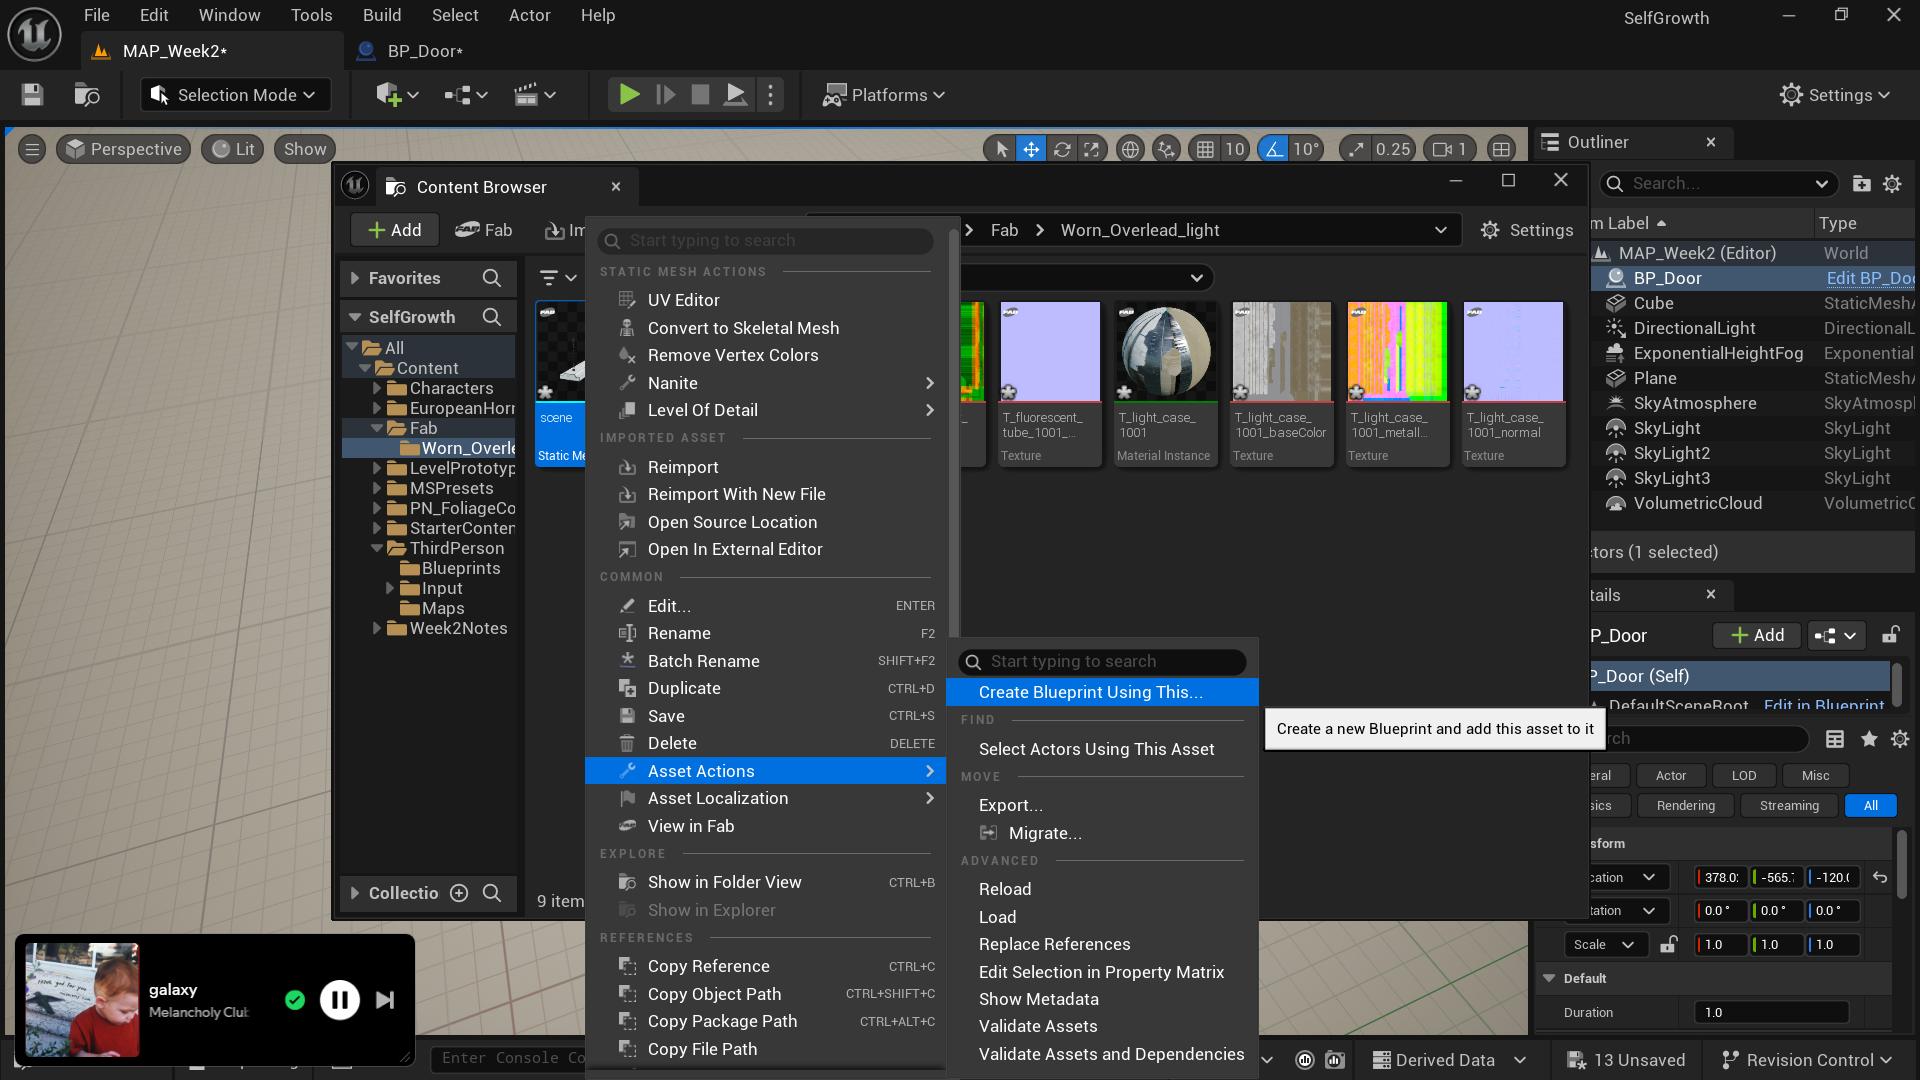
\includegraphics[width=1\linewidth]{day4images/screenshot013}
		\caption{A very quick to add functionality}
		\label{fig:screenshot013}
	\end{figure}
		\newpage
	In the Blueprint, I've added a rect.\ light as that resembles its real life behavior, which I then placed slightly below the light (change the source width and height to actually `scale' the light). I then added a sphere collider and placed it below the light, if our player is inside this volume, our light will turn on. (Change the Box Extent parameter here to properly scale the box.)
	
	\begin{figure}[h]
		\centering
		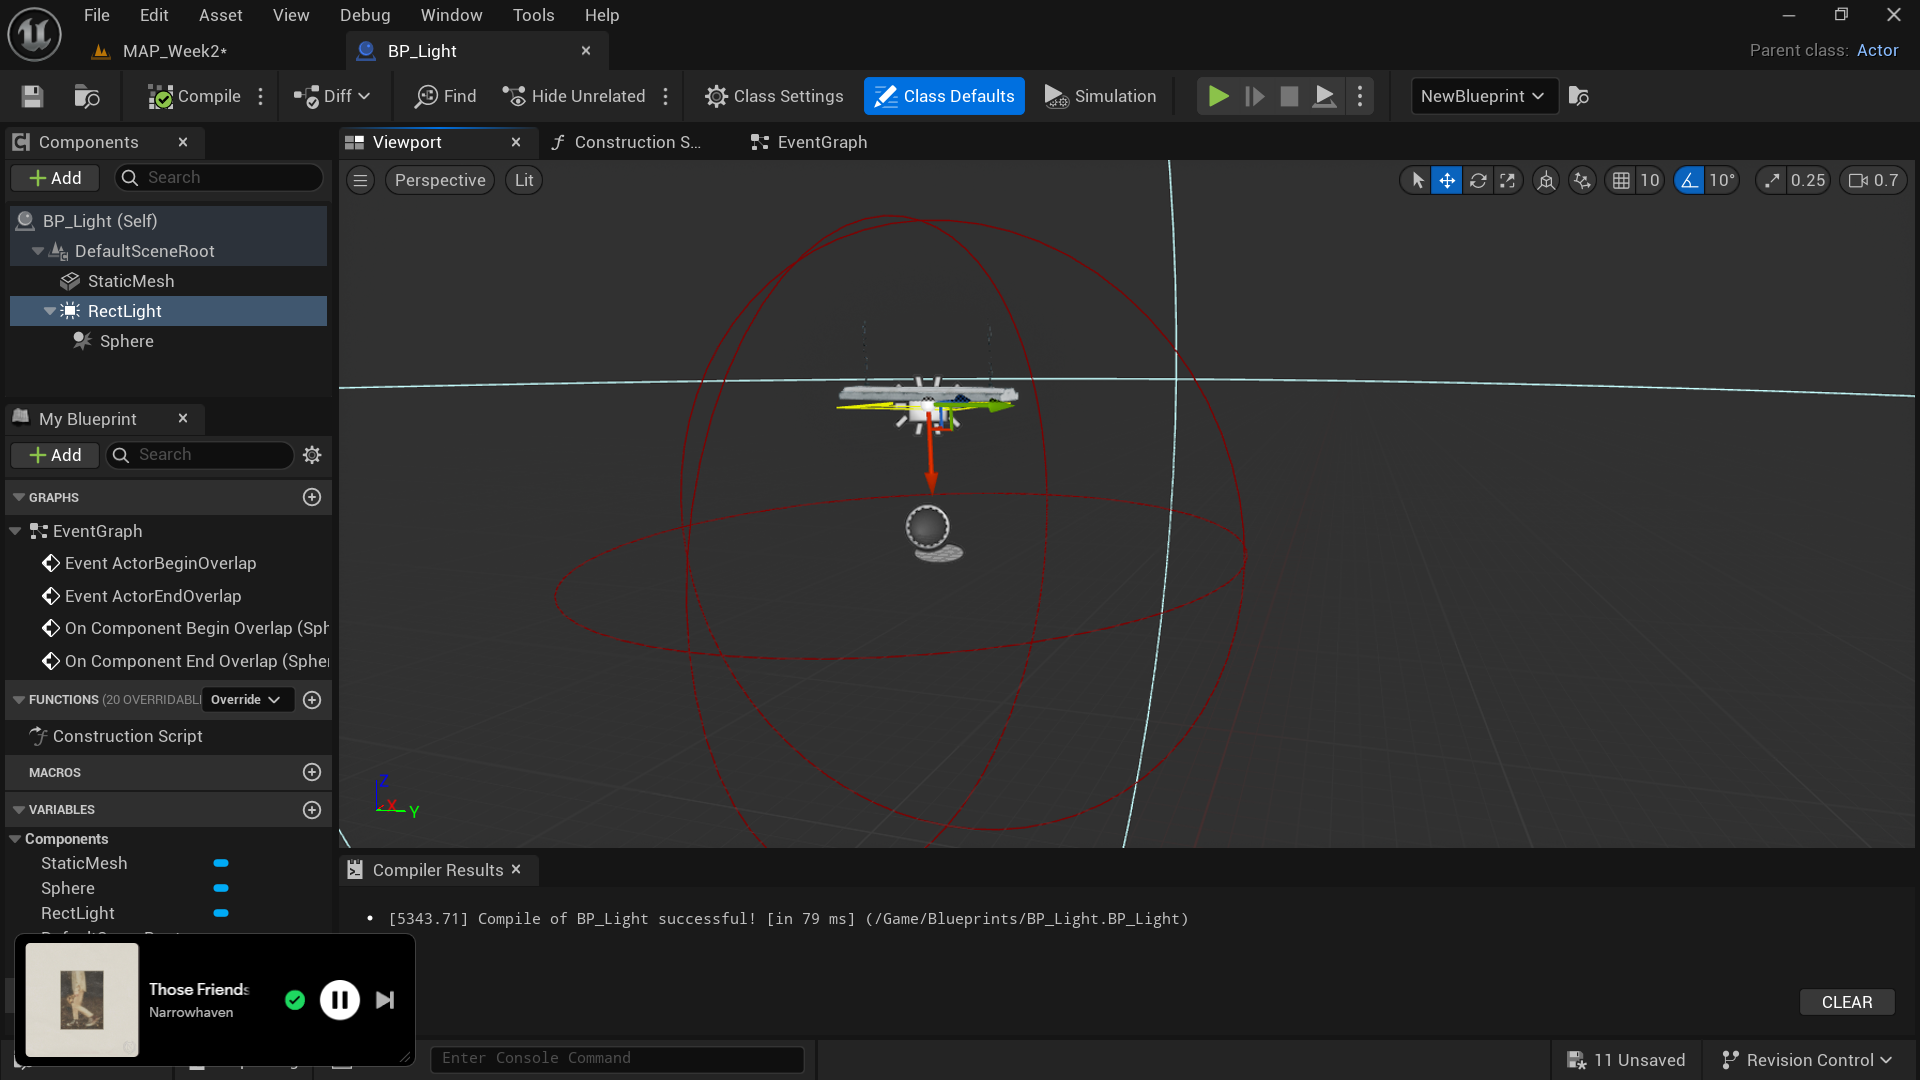
\includegraphics[width=1\linewidth]{day4images/screenshot015}
		\caption{BP\_Lights}
		\label{fig:screenshot015}
	\end{figure}

	Let's now head over to the Event Graph to add functionality to it. (Note, in the details panel of our light, there's an \verb*|Intensity| parameter, we'll be tweaking this.)
	
	
	\begin{figure}[h]
		\centering
		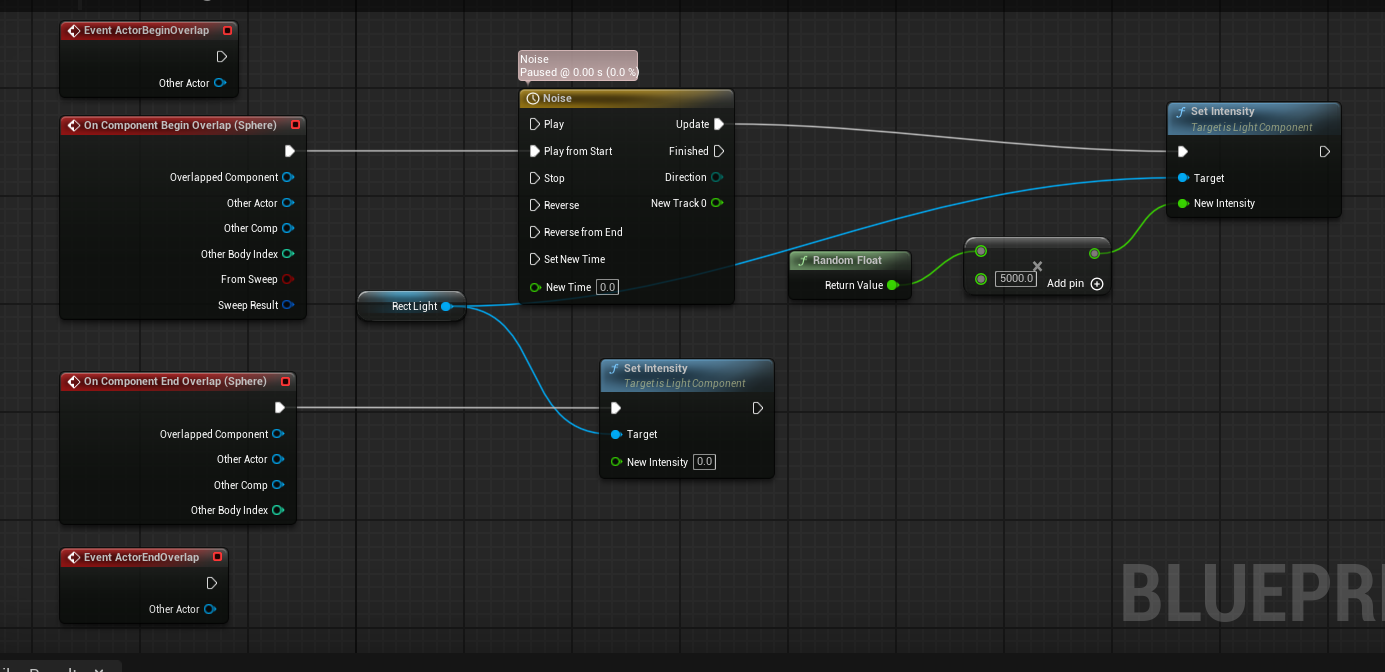
\includegraphics[width=1\linewidth]{day4images/screenshot016}
		\caption{On and off logic}
		\label{fig:screenshot016}
	\end{figure}
	\newpage
	Let me break this down.
	\begin{enumerate}
		\item Remember that by default the collision type is to send out an event per overlap (which does not block our character)
		\item Using either of the Event nodes I've grouped will give us the signal we're looking for (if we want our light to turn on only for a specific player, we can do that. More on this after)
		\item To spice things up (totally unnecessary, but fun), I'm randomly changing the intensity of our light when the player overlaps, maybe to simulate it turning on after a long time. Of course, it is very jittery (it changes the intensity every frame), a better way would be to perhaps add a delay node after a for-loop. This is just a proof of concept, you should experiment!
		\item The bigger red nodes are specific to the sphere collider we added (will only send a signal when we collided with \emph{only} this one.)
		\item If we also want our light to only turn on when a specific character comes closes (for example, not an AI), we do something referred to as casting, let's talk a little but about this now)
		\item An interesting gotcha is if you'd like this flickering to only happen once (the first time), connect the execution pin to \verb*|Play| instead of \verb|Play from Start|!
	\end{enumerate}
	
	\section{Blueprint Communication}
	It's a very common practice to want two (or more) different blueprints to want to communicate with each other. There are two ways to do so
	
	\begin{description}
		\item[Casting] Loading an entire blueprint into another to use it. It's recommended to keep the number of castings to a minimum, so we don't have to load an entire blueprint just to access a variable a ton of times.
		\item[Interfaces] A much more efficient way to access/manipulate functionality of another blueprint. 
	\end{description}
	
	A silly example: Starter Content ships with a Blueprint that does fire (Blueprint\_Effect\_Fire) (using Cascade, Unreal's old particle system. The newer one is Niagara). I will try to make something such that when the light is on, the fire will be off and vice versa. 
	\\[10pt]
	Take a look at the following:
	\begin{figure}[h]
		\centering
		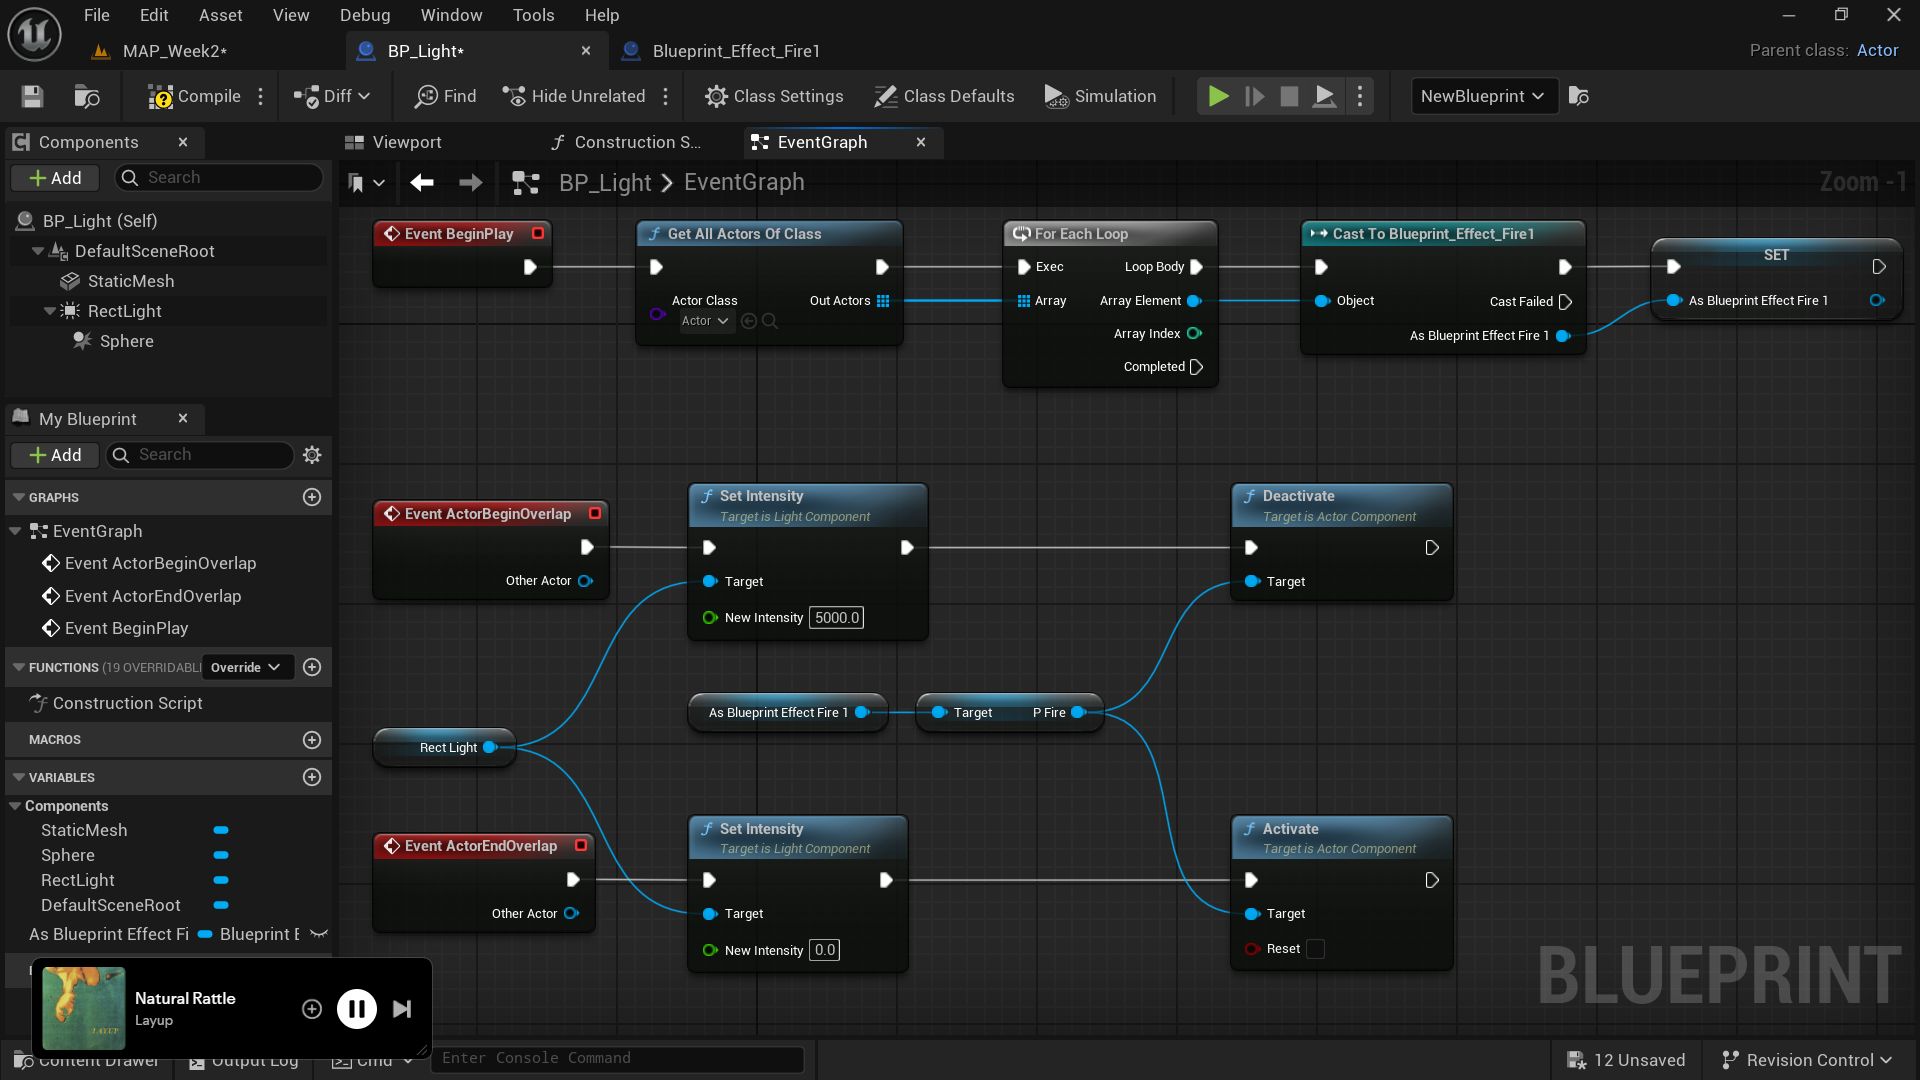
\includegraphics[width=1\linewidth]{day4images/screenshot017}
		\caption{Simple casting}
		\label{fig:screenshot017}
	\end{figure}
	
	
	
	Let me break down what I did.
	\begin{enumerate}
		\item Duplicated the \verb*|Blueprint_Effect_Fire| found in Starter Content \textgreater Blueprints. (Not necessary, but recommended, we will be making changes and it's helpful to have the original handy.)
		\item At the beginning of our game, we know the light will be off and our fire be on (this is will not always be the case, in that case it's necessary to use a \verb*|Validated Get|, right click a parameter and hit convert to validated get, this will only return the parameter if it exists).
		\item In our BP\_Light, using the Event BeginPlay I get a variable to the Blueprint\_Effect\_Fire1 (the duplicate we made) so I can access it's variables. 
		\begin{figure}[h]
			\centering
			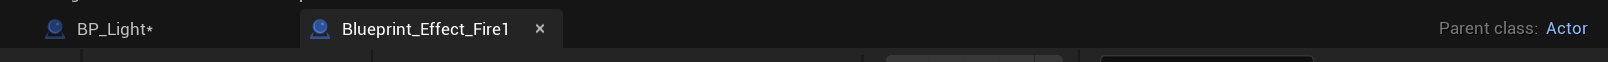
\includegraphics[width=1\linewidth]{day4images/screenshot018}
			\caption{Parent class of the fire blueprint}
			\label{fig:screenshot018}
		\end{figure}
		Since the parent class is an Actor (and not something that was meant to be interactive, like a Pawn or a Character), we'll have to loop through every actor whose parent is the Actor class and see if it's the one we need. This information is given by the \verb|Get All Actors of Class| node, by setting the \verb|Actor Class| parameter to \verb*|Actor| (the parent class we need). Indeed, I've said actor quite a few times, take a moment to make sense of this.\\[10pt] Using a for-each node we can iterate through the list we get. (See that the $3\times3$ symbol denotes it's an array.)\\[10pt] Casting this actor we got to the Blueptint\_Effect\_Fire1 (the blueprint we've actually dragged in our scene) will only be successful when we've found the correct actor. We can now store this parameter. (If we had used a for-each loop with break, we could've braked the loop here.) \\[10pt] We now have a reference to the blueprint we want to manipulate in this one! We can now \verb*|Activate| or \verb*|Deactivate| the fire as we please.\\[10pt] Note that we don't have to perform this casting and looping every time, we did it at the start and can now use this reference anytime any where.
		\item And that's pretty much it!
	\end{enumerate}
	
	\subsection{Using custom events}
	The last thing I'll talk about are custom events.
	
	\begin{figure*}[hb!]
		\centering
		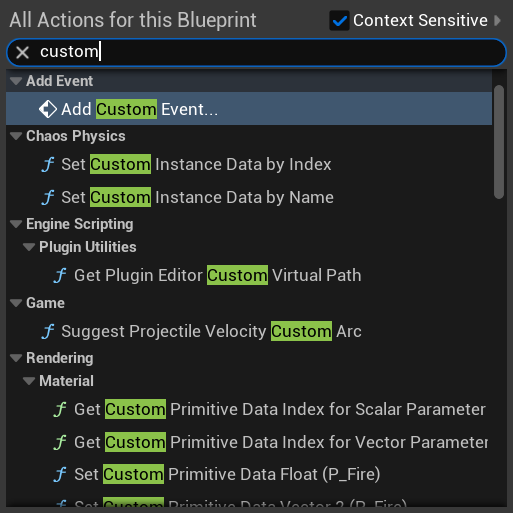
\includegraphics[width=0.55\linewidth]{day4images/screenshot019}
	\end{figure*}
	
	Take a look at the very tiny and well written \href{https://dev.epicgames.com/documentation/en-us/unreal-engine/custom-events-in-unreal-engine}{documentation for custom events} by Epic. They basically help us clean up our code a little bit and allow us to keep relevant functionality in their respective blueprints. For example, here, our logic for turning the fire on and off should be in blueprint that has the fire.
	
	\begin{figure}[h]
		\centering
		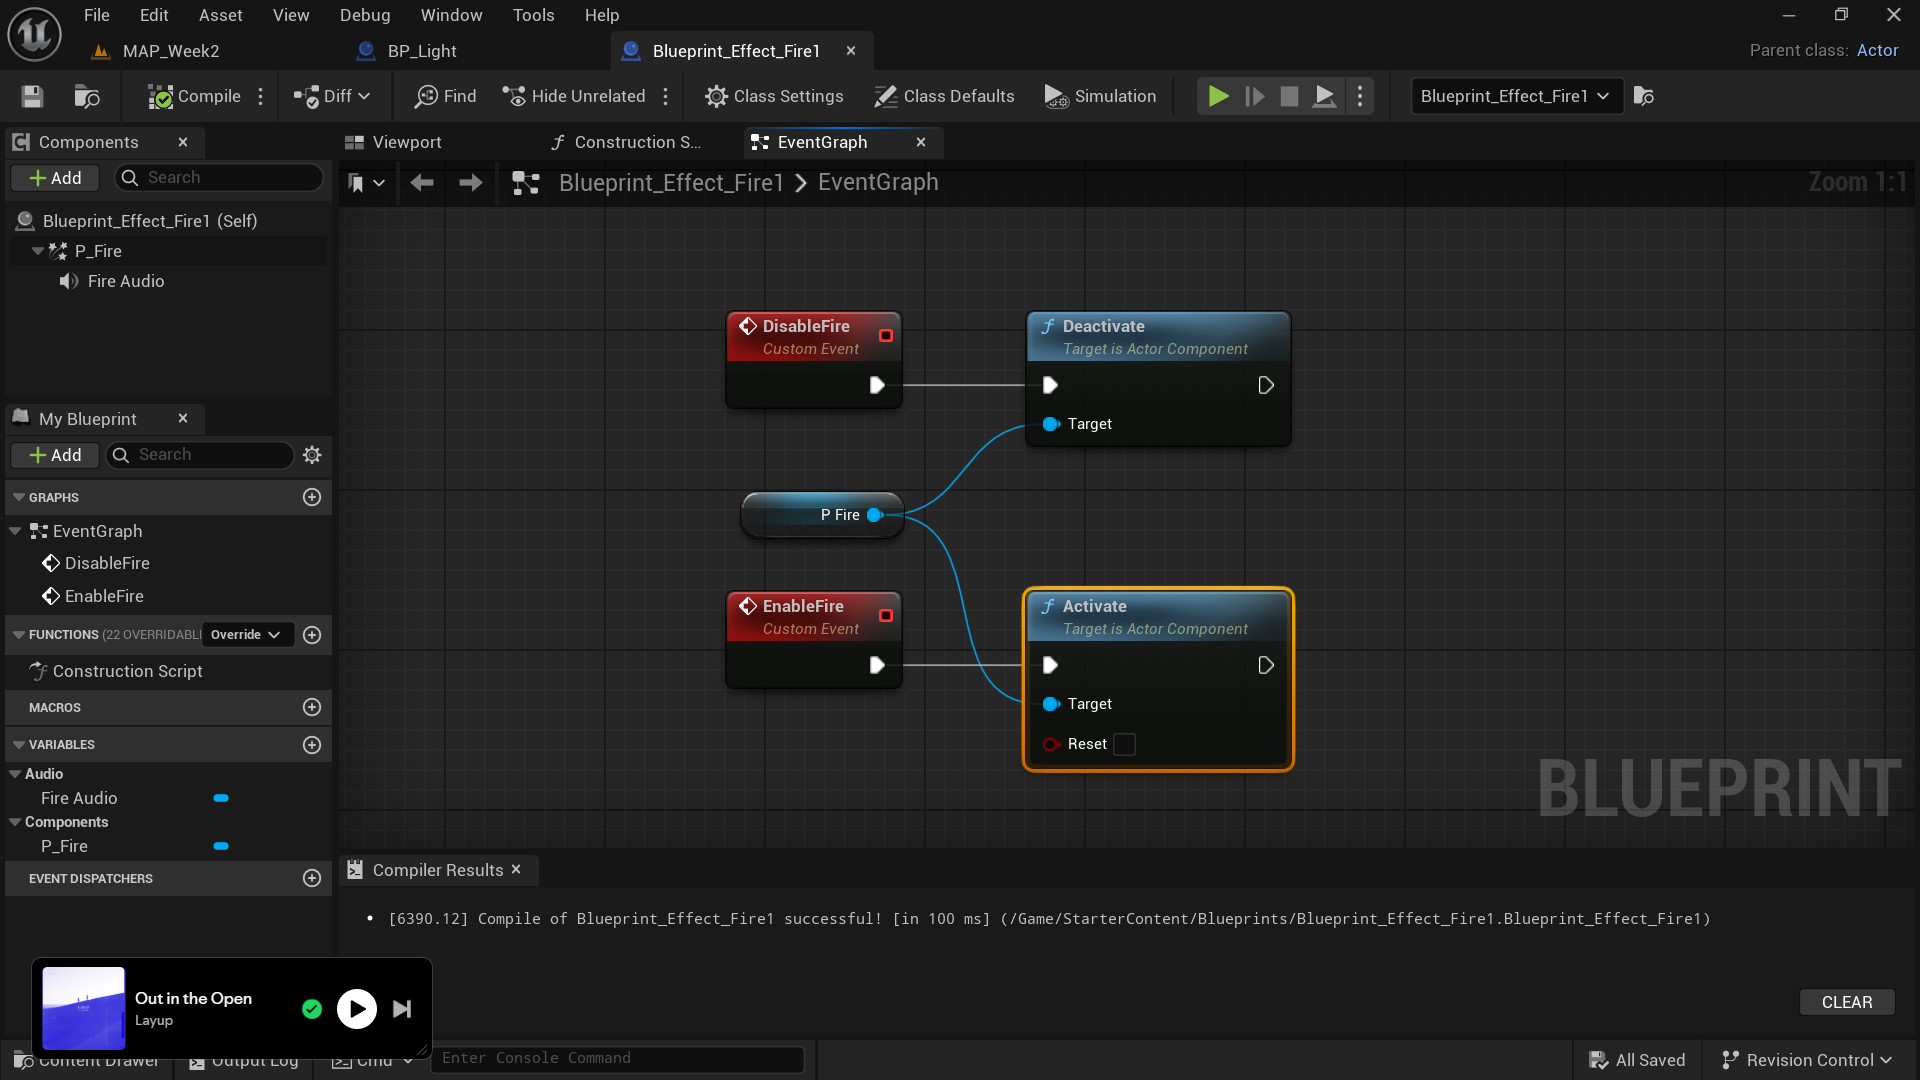
\includegraphics[width=0.8\linewidth]{day4images/screenshot020}
		\caption{(De)activating the fire using custom events in the fire blueprint}
		\label{fig:screenshot020}
	\end{figure}
	
	We will now activate these events in our blueprints with the lights, it's very simple to do so, just drag from our reference pin and type out the name you've given it.
	
	\begin{figure}[h]
		\centering
		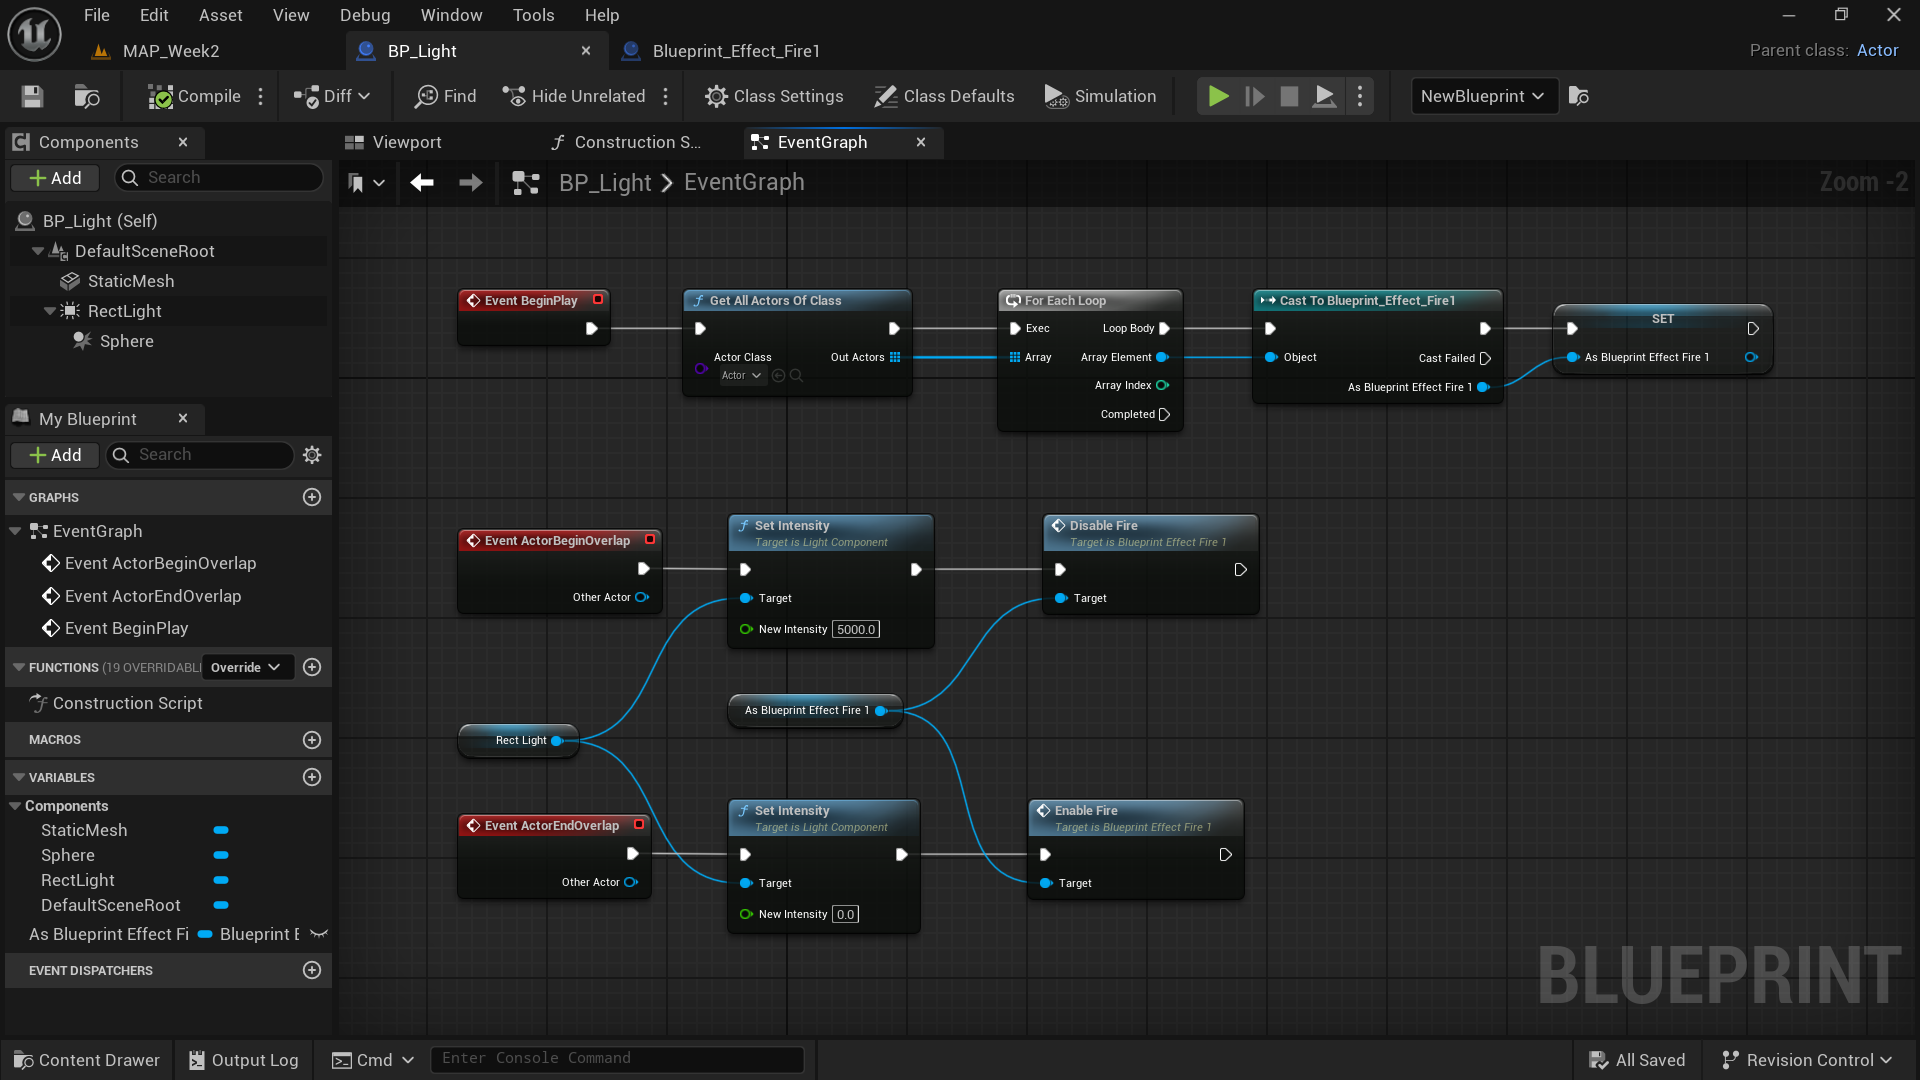
\includegraphics[width=0.8\linewidth]{day4images/screenshot022}
		\caption{Much cleaner}
		\label{fig:screenshot022}
	\end{figure}
	
	This allows us to keep things organized.
	
	\section{Conclusion}
	I will stop here, this probably feels very overwhelming right now, take a minute to walk through this, and I recommend recreating what I've created here. I'll give it out as a task:
	\\[10pt]
	\textbf{Task:} Make two blueprints. One that has lights which turn on and off based on proximity. The other which has fire. Control the state of the fire based on the status of lights. Using both custom events and without.
	\\[10pt]
	I believe I mentioned also talking about interfaces, I will not do that right now. It'll only delay these notes further, but they are important to talk about, I'll try to cover these some other time.
	In any case, if you've got any trouble following up, please let me know. It's important you let me know, there's no benefit to being stuck!
	
	
	
	
	
	
	
	
	
\end{document}